%!TEX root=main.tex
\section[Schädigung der Augen\hfill Umweltrelevante Phänomene und Prozesse]{Schädigung der Augen\\{\normalsize Umweltrelevante Phänomene und Prozesse}}
% https://de.wikipedia.org/wiki/Sehschw%C3%A4che
Schäden am visuellen System werden grob anhand der betroffenen Komponenten kategorisiert.

\subsection{Optische Fehlsichtigkeit (Ametropie)}


\paragraph{Kurzsichtigkeit (Myopie)}
\begin{quote}
\enquote{Beim \textit{kurzsichtigen} Auge liegt das Bild ferner Gegenstände \textit{vor} der Netzhaut. Zur Korrektur wird daher eine Zerstreuungslinse verwendet.} \cite[S. 236]{physik1}
\end{quote}

\begin{figure}
\centering
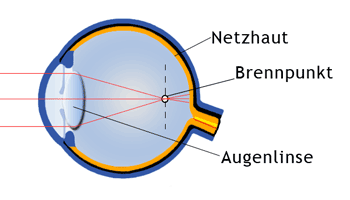
\includegraphics[width=4.5cm]{images/kurzsichtig.png}
\hspace{1cm}
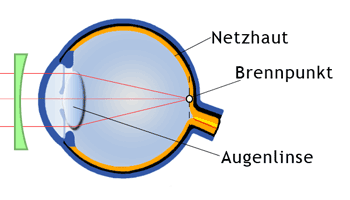
\includegraphics[width=4.5cm]{images/kurzsichtig_korrigiert.png}
\caption{Kurzsichtiges Auge \cite{abadi:fehlsichtigkeit}}
\end{figure}

Kurzsichtigkeit entsteht durch einen zu langen Augapfel oder eine zu starke Lichtbrechung, wodurch entfernte Objekte verschwimmen.

\paragraph{Weitsichtigkeit (Hyperopie)}
\begin{quote}
\enquote{Beim \textit{weitsichtigen} Auge liegt das Bild ferner Gegenstände \textit{hinter} der Netzhaut. Die Augenlinse muss also durch eine Sammellinse unterstützt werden.} \cite[S. 237]{physik1}
\end{quote}

\begin{figure}
	\centering
	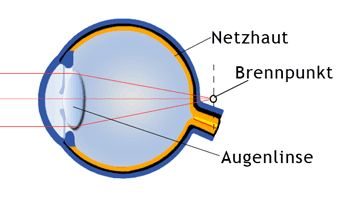
\includegraphics[width=4.5cm]{images/weitsichtig.png}
	\hspace{1cm}
	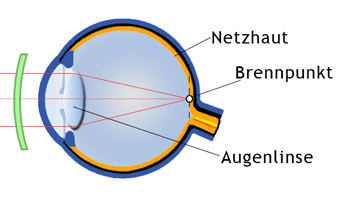
\includegraphics[width=4.5cm]{images/weitsichtig_korrigiert.png}
	\caption{Weitsichtiges Auge \cite{abadi:fehlsichtigkeit}}
\end{figure}

Weitsichtigkeit entsteht durch einen zu kurzen Augapfel, wodurch nahe Objekte verschwimmen.

Sie hängt nicht mit der Altersweitsichtigkeit zusammen, welche durch ein Nachlassen der Elastizität am Auge zustande kommt, wodurch Betroffenen kein scharfes sehen in der Nähe mehr möglich ist.

\newpage
\paragraph{Stabsichtigkeit (Astigmatismus)}
\begin{quote}
Beim \textit{stabsichtigen} Auge werden einfallende Lichtstrahlen unterschiedlich stark gebrochen und daher nicht in einem Punkt, sondern in einer Linie (Stab) abgebildet.
\end{quote}

\begin{figure}
	\centering
	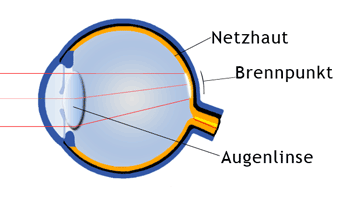
\includegraphics[width=4.5cm]{images/stabsichtig.png}
	\caption{Stabsichtiges Auge \cite{abadi:fehlsichtigkeit}}
\end{figure}

Stabsichtigkeit entsteht meist durch eine Hornhautverkrümmung und führt zu einem verzerrten oder verschobenen Bild.
